\documentclass[12pt]{article}

% Paketi za podršku jeziku, matematici i slikama
\usepackage[utf8]{inputenc}
\usepackage[T1]{fontenc}
\usepackage[serbian]{babel}
\usepackage{amsmath}
\usepackage{graphicx}
\usepackage{hyperref}
\usepackage{geometry}
\geometry{a4paper, margin=1in}

% Naslov dokumenta
\title{Predviđanje koncentracije PM2.5 čestica primjenom modela vremenskih serija i dekompozicije trenda}
\author{}
\date{}

\begin{document}
	
	\maketitle
	
	\section{Opis problema}
	Kvalitet vazduha u urbanim sredinama direktno zavisi od složene interakcije između antropogenih faktora (individualna ložišta, saobraćaj, industrija) i meteoroloških prilika. Koncentracija zagađivača poput PM2.5 čestica nije slučajan broj, već podatak koji prati jasne hronološke obrasce. Problem koji ovaj projekat rješava je predviđanje budućih vrijednosti zagađenja na osnovu istorijskih podataka.
	
	Ključni pojmovi analize:
	\begin{itemize}
		\item \textbf{Sezonalnost:} Kako se zagađenje mijenja ciklično (npr. grejna sezona naspram ljetnjeg perioda).
		\item \textbf{Trend:} Analiza da li se opšti kvalitet vazduha pogoršava ili poboljšava kroz godine.
		\item \textbf{Ciklične varijacije:} Promjene unutar jednog dana, poput jutarnjih i popodnevnih špiceva.
	\end{itemize}
	
	\begin{figure}[h]
		\centering
		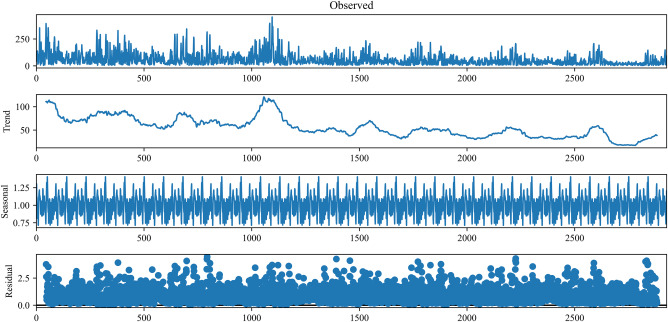
\includegraphics[width=\textwidth]{primjer1.jpg} 
		\caption{Rezultati jednog sličnog projekta}
	\end{figure}
	
	\section{Skup podataka (Dataset)}
	\textbf{Izvor:} UCI Machine Learning Repository - Beijing Multi-Site Air-Quality, dostupan i na platformi Kaggle.
	
	\textbf{Opis skupa:} Ovaj skup sadrži satna mjerenja zagađenja vazduha sa 12 različitih mjernih stanica u Pekingu u periodu od nekoliko godina. Fokus će biti na podacima sa jedne specifične stanice (npr. Aotizhongxin) kako bi se analizirala jedna vremenska serija.
	
	\section{Metodologija}
	Proces rješavanja problema biće podijeljen u četiri ključne faze:
	
	\subsection*{I Faza: Pretprocesiranje i numerička obrada podataka}
	Vremenske serije ne trpe NaN, stoga je prvi korak rješavanje nedostajućih vrijednosti.
	\begin{itemize}
		\item \textbf{Vremensko usklađivanje:} Konverzija kolona (year, month, day, hour) u jedinstveni datetime objekat koji će služiti kao indeks.
		\item \textbf{Linearna interpolacija:} Koristiće se numerička linearna interpolacija za popunjavanje NaN vrijednosti, čime se čuva kontinuitet serije.
	\end{itemize}
	
	\subsection*{II Faza: Eksplorativna analiza i statistički testovi}
	Prije modelovanja neophodno je analizirati podatke:
	\begin{itemize}
		\item \textbf{Dekompozicija:} Razlaganje serije na trend, sezonalnost i reziduale (šum) korišćenjem biblioteke \texttt{statsmodels}.
		\item \textbf{Provjera stacionarnosti:} Primjena Augmented Dickey-Fuller (ADF) testa kako bi se utvrdilo da li su statistička svojstva serije stabilna.
		\item \textbf{Korelaciona analiza:} Provjera uticaja spoljnih faktora (brzina vjetra, temperatura) na koncentraciju čestica.
	\end{itemize}
	
	\subsection*{III Faza: Modelovanje (Poređenje modela)}
	Implementiraće se dva pristupa radi poređenja:
	\begin{itemize}
		\item \textbf{ARIMA (AutoRegressive Integrated Moving Average):} Klasični statistički model baziran na linearnoj kombinaciji sopstvenih prethodnih vrijednosti i grešaka.
		\item \textbf{Random Forest Regressor:} Metoda mašinskog učenja gdje se prošle vrijednosti ($t-1, t-2$) koriste kao ulazni atributi.
		\item \textbf{Napomena:} Postoji mogućnost male promjene algoritama zato što mi nije još u potpunosti poznata njihova implementacija.
		
	\end{itemize}
	
	\section{Način evaluacije}
	Rezultati će se evaluirati na testnom skupu (posljednjih 20\% podataka). Koristiće se numeričke metrike:
	\begin{itemize}
		\item \textbf{RMSE (Root Mean Square Error):} Daje veću težinu velikim greškama:
		\[ RMSE = \sqrt{\frac{1}{n}\sum_{i=1}^{n}(y_i - \hat{y}_i)^2} \]
		\item \textbf{MAE (Mean Absolute Error):} Prosječno odstupanje u mikrogramima ($\mu\text{g/m}^3$).
		\item \textbf{Vizuelna evaluacija:} Grafik koji preklapa stvarnu i predviđenu krivu zagađenja.
	\end{itemize}
	
	\section{Tehnologije}
	\begin{itemize}
		\item \textbf{Programski jezik:} Python 3.x.
		\item \textbf{Biblioteke za obradu:} \texttt{Pandas} i \texttt{NumPy}.
		\item \textbf{Statistika i ML:} \texttt{Statsmodels} i \texttt{Scikit-learn}.
		\item \textbf{Vizuelizacija:} \texttt{Matplotlib} ili \texttt{Seaborn}.
	\end{itemize}
	
	\section{Literatura}
	\begin{itemize}
		\item Kaggle - Beijing Air Quality Analysis \href{https://www.kaggle.com/datasets/sid321axn/beijing-multisite-airquality-data-set}{[Link]}.
		\item Air Quality Prediction using Machine Learning \href{https://github.com/topics/air-quality-prediction}{[Link]}.
		\item Istraživački rad (ScienceDirect): \textit{Forecasting of Beijing PM2.5 with a hybrid ARIMA model...}.
	\end{itemize}
	
\end{document}